\subsection{\ac{rltanlage} Vergangenheit}
Lüftungsgeräte sind schon seit längerer Zeit in Verwendung \zB in Wirtschaftsbetrieben, Gastronomie aber auch in Bürogebäuden. Die Ursprünge von Lüftungsgeräten bzw. \ac{rltanlage} lassen sich jedoch schon auf ca. 3000 v. Chr. datieren.
Die ersten Versuche fanden dahingehen Anwendung, um Höhlen und Unterkünfte vom Rauch des Feuers zu befreien. Es wurden solche Arten von Raumbelüftungen \zB in Ondol in Alaska gefunden.
Lüftungstechnik wurde damals durch den natürlichen Wetterzyklus bestimmt. 
Erst im späteren Verlauf wurde, durch die Entwicklung moderner Belüftungs- und Klimatechnik, die aktive Belüftung- und Temperaturregelung möglich.

Die ersten Gehversuche einer richtigen \acs{rltanlage} wurde 1836 im House of Commons in London gemacht. Die Anlage umfasst alle Punkte einer \acs{rltanlage}: Heizen, Kühlen, Be- und Entfeuchten sowie Filtern der Luft. 

Die Anlage versorgte das House of Commons mit Zuluft welche links unten bei den Gitter angesaugt wird (Die Ansaugung der Frischluft lag knapp über der Themse). Die Kühlung wurde durch Eis welches in der Kammer hinter den Gittern liegt realisiert.
Die Filterung wurde durch Baumwolle, welche bei Punkt C aufgeschichtet wird realisiert.
Nach der Filterung wurde beim Punkt A die Luft erhitzt. 
Danach strömte die Luft durch den doppelten Boden und wurde dadurch verteilt. Die Luft strömte nun nach oben und wurde bei Punkt F aus dem Gebäude geleitet. Im Winter leitete man die Luft nach links direkt aus dem Fenster geleitet. Im Sommer hingegen wurde die Luft nach rechts durch die Verrohung und durch den Kamin  nach draußen geleitet. 
(siehe Abb.~\ref{fig:House_of_Commons_Klimatechnik}).
\cite{Fitzner_Finke:2010} 

\begin{figure}[ht]
	\centering
	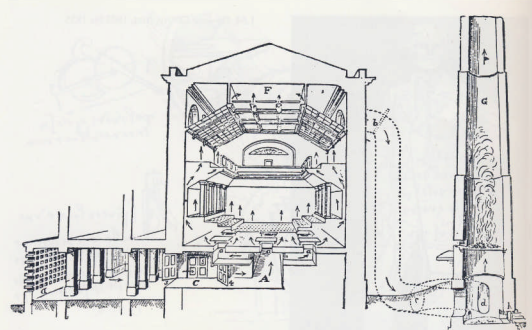
\includegraphics[width=0.6\linewidth]{Bilder/Belueftung_House_of_Commons}
	\caption{Klimatechnik House of Commons  (Quelle: \url{https://vhkk.org/page/vortrag/pdf/Geschichte_Raumklimatechnik.pdf})}
	\label{fig:House_of_Commons_Klimatechnik}
\end{figure}



\subsection{\ac{rltanlage} Gegenwart}
Die Funktionen einer \ac{rltanlage} unterscheidet sich Grundsätzlich nicht wirklich von dem was schon z.B. 1836 im House of Commons in London verwendet wurde. Die einzelnen Abschnitte wie \zB Ansaugung, Filtration, Be- und Entfeuchtung, Kühlung, Heizung und Absaugung haben sich, in deren Funktionen, wenig verändert. Der Aufbau, die Funktionsweise und die Umsetzung der einzelnen Abschnitte änderte sich  grundlegend.

Der Aufbau im Generellen hat sich dahingehend restrukturiert, dass eine moderne \ac{rltanlage} sehr kompakt im Aufbau ist. Angefangen bei den Steuerungsklappen für Zu- bzw. Abluft über die Ventilatoren, das Heiz- bzw. Kühlregister, die Wärmerückgewinnungsanlage, die Filter und den Luft Be- und Entfeuchter, ist alles in einer \ac{rltanlage} untergebracht.
Die \ac{rltanlage} wird von außen mit leichten Aluminiumplatten verkleidet, welche von innen Schall- und Wärme-isoliert sind. Dies ist dahingehend wichtig, da die \acp{rltanlage} meist außerhalb, \zB auf Dächern oder hinter dem Haus angeschlossen werden. 







\subsection{Überlegungen (vor Abgabe LÖSCHEN!!!)} 

Vergangenheit (Aufbau)
Gegenwart (Aufbau: Gerät von Aussen) --> Komponenten fehlen noch
---------------------------------------------------------
-funktion (allgemein, Gerät tdot, walter bösch geräte)
wichtigkeit 
-Wichtig: Gesundheit, Wohlbefinden etc.
Einsetzgebiete: betriebe, büros, gastronomie

